\newcommand{\booktitle}{用户手册}
\newcommand{\tocname}{目录}
\newcommand{\chapword}{第 \thesection\ 章}
\documentclass[11pt,a4paper]{article}
\usepackage[top=20mm,bottom=21mm,left=22mm,right=22mm,headheight=16pt,footskip=11mm]{geometry}
\usepackage{fontspec,xeCJK,graphicx,xcolor,tabularx,array,booktabs,enumitem,fancyhdr,hyperref}
\setmainfont{TeX Gyre Pagella}
\setsansfont{TeX Gyre Heros}
\setmonofont[Scale=.89]{Latin Modern Mono}
\IfFileExists{C:/Windows/Fonts/msyh.ttc}
{\setCJKmainfont[AutoFakeBold=2]{SimSun}\setCJKsansfont{Microsoft YaHei}\setCJKmonofont{Microsoft YaHei}}
{\setCJKmainfont[BoldFont=FandolSong-Bold.otf]{FandolSong-Regular.otf}\setCJKsansfont[BoldFont=FandolHei-Bold.otf]{FandolHei-Regular.otf}\setCJKmonofont{FandolHei-Regular.otf}}
\definecolor{ink}{HTML}{18373A}\definecolor{teal}{HTML}{006B64}
\definecolor{muted}{HTML}{496164}\definecolor{wash}{HTML}{EAF4F0}\definecolor{linecolor}{HTML}{A3C0B6}
\hypersetup{unicode=true,colorlinks=true,linkcolor=teal,urlcolor=teal,bookmarksnumbered=true,pdftitle={IM Tool — \booktitle},pdfauthor={IM Tool}}
\setlength{\parindent}{0pt}\setlength{\parskip}{6pt}\linespread{1.09}
\setlist[enumerate]{leftmargin=1.85em,itemsep=3pt,topsep=2pt,parsep=0pt,label=\textcolor{teal}{\sffamily\bfseries\arabic*.}}
\raggedbottom\setlength{\emergencystretch}{2em}
\pagestyle{fancy}\fancyhf{}\fancyhead[L]{\sffamily\bfseries\color{teal} IM Tool}
\fancyhead[R]{\small\sffamily\color{muted}\nouppercase{\leftmark}}
\fancyfoot[L]{\footnotesize\sffamily\color{muted}\booktitle\enspace ·\enspace 1.2.4}
\fancyfoot[R]{\sffamily\bfseries\color{teal}\thepage}
\renewcommand{\headrule}{{\color{linecolor}\hrule height .65pt width\headwidth}}
\renewcommand{\contentsname}{\tocname}
\newcommand{\code}[1]{{\ttfamily\detokenize{#1}}}
\newcommand{\ui}[1]{{\sffamily\bfseries\color{ink}#1}}
\newcommand{\chapterpage}[2]{\clearpage\refstepcounter{section}\label{#1}\markboth{#2}{}%
\addcontentsline{toc}{section}{\protect\numberline{\thesection}#2}%
{\sffamily\bfseries\color{teal}\chapword\par}\vspace{1mm}%
{\raggedright\sffamily\bfseries\fontsize{23}{29}\selectfont\color{ink}#2\par}\vspace{2mm}}
\newcommand{\subhead}[1]{\par\addvspace{2mm}{\large\sffamily\bfseries\color{teal}#1\par}\nobreak}
\newcommand{\note}[2]{\par\smallskip\colorbox{wash}{\parbox{\dimexpr\linewidth-2\fboxsep\relax}{\raggedright\vspace{1mm}\sffamily\textbf{\color{teal}#1}\enspace#2\vspace{1mm}}}\par}
\newcommand{\tbl}[3]{\par\smallskip\begingroup\small\renewcommand{\arraystretch}{1.23}
\begin{tabularx}{\linewidth}{@{}>{\raggedright\arraybackslash}p{.30\linewidth}>{\raggedright\arraybackslash}X@{}}
\toprule\sffamily\bfseries\color{teal}#1&\sffamily\bfseries\color{teal}#2\\\midrule #3\bottomrule\end{tabularx}\endgroup\par}
\newcommand{\pic}[3]{\par\smallskip\begingroup\centering\includegraphics[width=\linewidth,height=#3,keepaspectratio]{figures/#1.png}\par\endgroup{\small\color{muted}#2\par}\smallskip}
\newcommand{\cover}[3]{\thispagestyle{empty}\vspace*{12mm}
\includegraphics[width=29mm]{../../im_app/resources/im-tool.png}\par\vspace{12mm}
{\sffamily\bfseries\fontsize{50}{54}\selectfont\color{ink}IM Tool\par}\vspace{3mm}
{\sffamily\bfseries\fontsize{28}{34}\selectfont\color{teal}\booktitle\par}\vspace{4mm}
{\Large\color{muted}#1\par}\vfill
\begin{flushleft}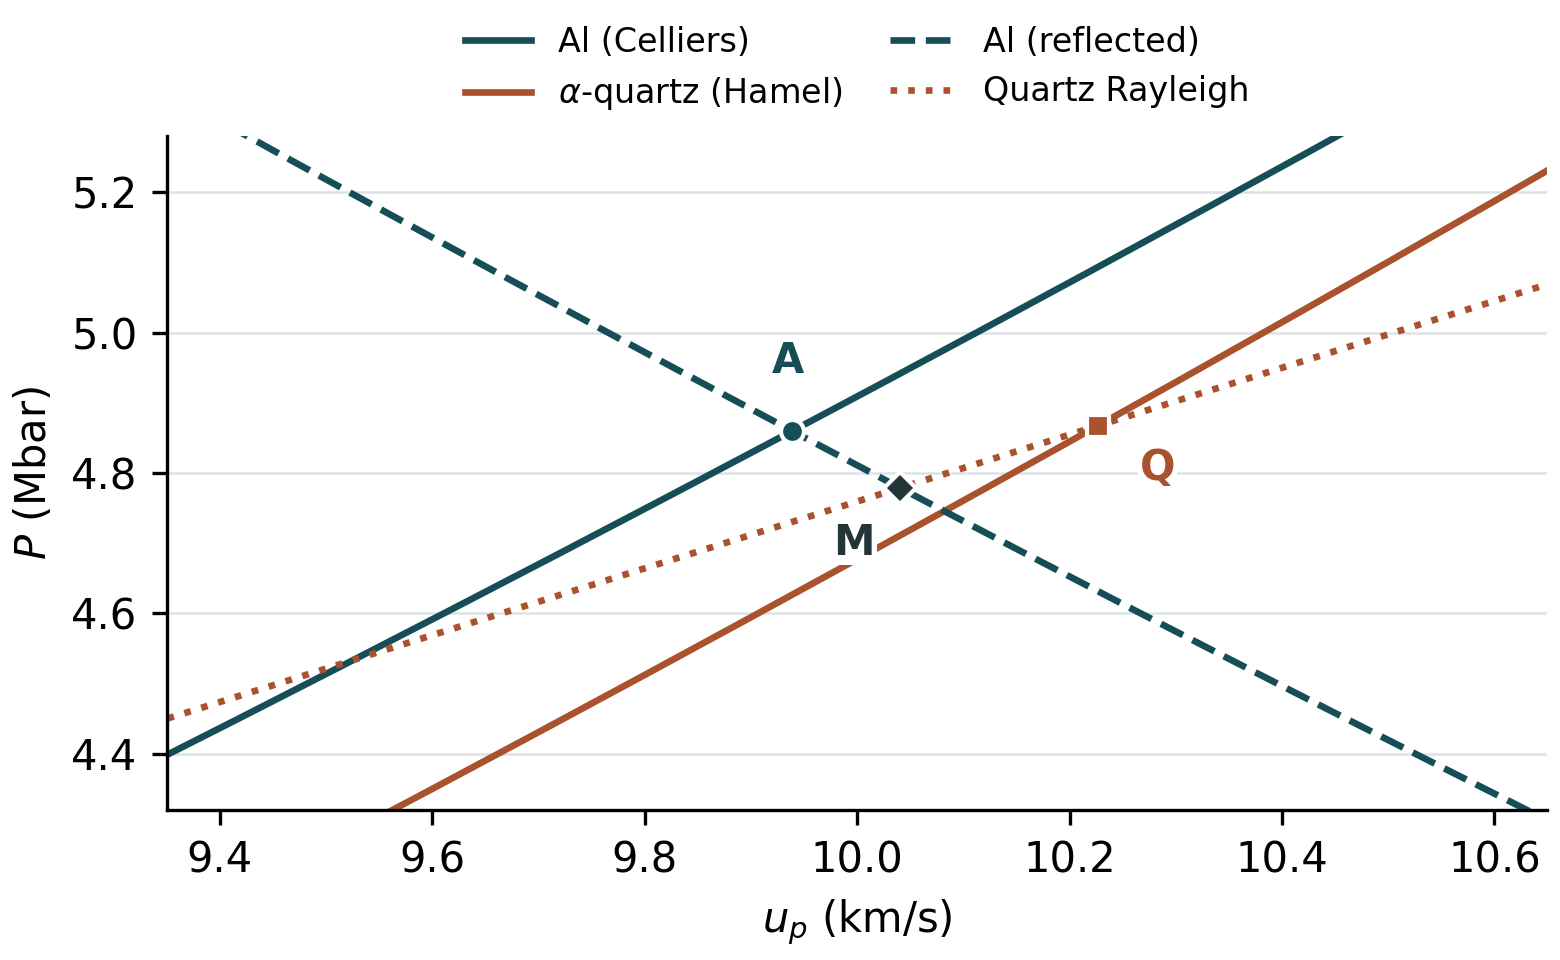
\includegraphics[width=.67\linewidth,height=81mm,keepaspectratio]{figures/tutorial-plot.png}\end{flushleft}
{\small\color{muted}#2\par}\vfill{\color{linecolor}\rule{\linewidth}{.7pt}}\par
{\large\sffamily\bfseries\color{ink}#3}\hfill{\sffamily\color{muted}2026.11}\clearpage}

\begin{document}\color{ink}
\cover{阻抗匹配与材料数据可视化}{Hicks 第 29400 号实验。A、Q 分别由实测冲击波速度和 Celliers 铝、Hamel 石英拟合得到。M 是由铝的镜像 Hugoniot 与石英瑞利线求得的界面状态。}{桌面版 1.2.4\enspace ·\enspace 徐博}
\phantomsection\pdfbookmark[1]{目录}{contents}\markboth{目录}{}\tableofcontents
\subhead{第一次使用}
从 \ui{Help → Open Practice Workspace} 打开练习。第~\ref{workspace}、\ref{crossing}~章用 Hicks 第 29400 号实验的两个实测冲击波速度，读出 Celliers 铝和 Hamel 石英上的状态，再求界面压强。拟合公式和原文见第~\pageref{sources}~页。
\note{界面语言}{手册保留软件控件的英文原名，便于按文字定位。安装页截图来自 Windows 简体中文向导，数据分析截图来自 Ubuntu 上的 Qt 桌面程序。}

\chapterpage{windows}{在 Windows 上安装}
\begin{enumerate}
\item 在 64 位 Windows 10 或 11 上，双击 \code{IM-Tool-Setup-1.2.4-x64.exe}，在语言选择框中选择简体中文或英语。
\item 阅读欢迎页，选择安装位置。默认目录为 \verb|%LOCALAPPDATA%\Programs\IM Tool|。软件按当前 Windows 用户安装，程序包包含 Python、Qt 和绘图库。
\item 按需勾选“创建桌面快捷方式”，点击“安装”。完成页可勾选启动 IM Tool 立即运行，以后也可在“开始”菜单中搜索 \ui{IM Tool}。
\item 打开软件的 \ui{Help} 菜单，选中文版或英文版手册，系统会使用本机 PDF 阅读器打开。选择 \ui{Open Practice Workspace} 可进入练习。
\end{enumerate}
\pic{wizard-zh}{Windows 简体中文欢迎页。点击“下一步”后可以选择安装目录，并决定是否创建桌面快捷方式。}{77mm}
\subhead{首次启动会在哪里写入文件}
首次启动时，程序将随包材料库复制到用户目录。点击 \ui{Help → Open Working Folder} 可直达当前 \code{standard_library} 文件夹。同级的 \code{workflows} 是保存 JSON 工作流的默认目录。铝和石英练习的材料库和工作流位于 \code{Practice/Celliers-Hamel}。
\subhead{升级和卸载}
升级前关闭 IM Tool 的所有窗口，再启动新版安装程序，选择原安装目录。程序和随包手册会更新。已有的用户材料库会继续使用，其中可以保存自己添加的表格。要卸载程序，进入 Windows“设置 → 应用 → 已安装的应用”，选择 IM Tool 并卸载。工作文件保存在用户目录，可单独备份。
\note{安装后检查}{确认能看到交叉曲线图标、九个绘图标签页和 Help 菜单。初次打开时画布可以为空，勾选材料后才会出现相应曲线。}

\chapterpage{linux}{在 Linux 上安装}
按发行版选包。在图形文件管理器中用系统的软件安装器打开本地软件包，查看依赖后点击安装。若双击打开了压缩包查看器，可右键选择“打开方式”并改用软件安装器，也可在下载目录中运行相应命令。
\tbl{发行版}{安装文件和命令}{
Debian、Ubuntu & \code{im-tool_1.2.4-1_all.deb}\\[-1pt]
& \code{sudo apt install ./im-tool_1.2.4-1_all.deb}\\
Fedora & \code{im-tool-1.2.4-1.noarch.rpm}\\[-1pt]
& \code{sudo dnf install ./im-tool-1.2.4-1.noarch.rpm}\\}
Linux 安装包使用发行版提供的 Python 3、PyQt5、绘图库及电子表格读取库。安装时若缺依赖，包管理器可能需要访问软件源。安装完成后，桌面程序、两份手册和练习表格均可离线使用。
\subhead{启动和检查}
进入图形桌面，在应用菜单中搜索 \ui{IM Tool}，也可在终端运行 \code{im-tool}。若程序未能启动，从终端启动可以看到第一条错误信息。通过远程终端运行 Qt 程序时，需要已配置的图形显示环境。
\subhead{定位文件、升级和卸载}
系统程序位于 \code{/usr/share/im-tool/}。用户文件默认在 \verb|~/.local/share/IM Tool/| 下。设置了 \code{XDG_DATA_HOME} 时会使用其对应目录。可从 \ui{Help → Open Working Folder} 查看正在使用的库。升级时用同一包管理器安装新版文件。如果是同一版号的重新构建，可用 \code{apt reinstall} 或 \code{dnf reinstall} 加本地文件路径重装。卸载可用 \code{sudo apt remove im-tool} 或 \code{sudo dnf remove im-tool}。
\note{检查已安装版本}{Debian 和 Ubuntu 使用 \code{dpkg-query -W im-tool}，Fedora 使用 \code{rpm -q im-tool}。平时以普通用户启动桌面程序，创建的工作文件就属于当前账户。}

\chapterpage{workspace}{载入 Celliers 铝和 Hamel 石英}
打开 \ui{Help → Open Practice Workspace}。材料列表已勾选 \ui{Aluminum} 和 \ui{Alpha Quartz}。对应的 ID 为 \code{Al_Celliers2005} 和 \code{Quartz_Hamel2012}，各含 500 个拟合采样点。
\begin{enumerate}
\item 在 \ui{Rayleigh Lines} 中核对 Hicks 等人表 I 第 29400 号实验的实测冲击波速度。铝的 $D=18.11\pm0.32$ km/s、$\rho_0=2.70$ g/cm³，石英的 $D=17.96\pm0.26$ km/s、$\rho_0=2.65$ g/cm³。双击已载入的直线可以查看参数。
\item 在 \ui{Find Intersection} 中选择 \ui{Aluminum} 与铝的 \ui{Rayleigh} 条目（$D=18.11$），点击同名按钮。得到铝初始冲击态 A，粒子速度为 9.9390 km/s，压强为 4.8599 Mbar。
\item 改选 \ui{Alpha Quartz} 与石英的 \ui{Rayleigh} 条目（$D=17.96$），再次求交。由 Hamel 拟合得到石英状态 Q，读数为 10.2267 km/s、4.8673 Mbar。保留这两行，供下一章核对。
\end{enumerate}
\pic{workspace}{打开练习后，图中显示两条拟合 Hugoniot 和两条由实测波速给定的瑞利线。坐标范围已放大到第 29400 号实验所在区域。}{78mm}
\note{怎样辨认结果行}{手册按求交顺序把三行称为 A、Q 和 M，界面会分配自己的交点 ID。可从练习窗口的 \ui{Help → Open Working Folder} 查看两份原始材料文件。}

\chapterpage{crossing}{求铝与石英的界面状态}
\begin{enumerate}
\item 在 \ui{Reflect / Release} 中将 \ui{Curve} 设为 \ui{Aluminum}。\ui{About intersection} 选择上一章的铝状态 A（$u_p=9.9390$ km/s），点击 \ui{Reflect}，程序将围绕该粒子速度生成 Celliers 铝的镜像曲线。
\item 在 \ui{Find Intersection} 中选择 \code{Reflected Al_Celliers2005} 与 \code{Quartz_Hamel2012} 的 \ui{Rayleigh} 线（$D=17.96$）。点击求交，结果行 M 给出 $u_p=10.0405$ km/s、$P=4.7787$ Mbar，即 477.87 GPa。
\item 核对 Hicks 表 I。论文推得 10.07 km/s、4.79 Mbar，压强的随机不确定度为 0.17 Mbar，系统不确定度为 0.04 Mbar。上一章的 Q（4.8673 Mbar）来自石英实测波速与 Hamel 拟合，可与 M 对照。
\end{enumerate}
\pic{intersection}{选中的第三行由铝镜像曲线与石英瑞利线求得，前两行分别对应铝和石英各自的主 Hugoniot。}{76mm}
\subhead{怎样理解镜像近似}
对于铝曲线上的每个点，软件保持压强不变，将粒子速度变换为 $u_p'=2u_{p,A}-u_p$，以此近似铝的卸载路径。采用 g/cm³ 和 km/s 时，石英瑞利线满足 $P\,(\mathrm{Mbar})=0.01\rho_0 D u_p$。
\note{区分读数的来源}{实验直接给出两个冲击波速度。论文的界面压强和本章复算的压强均依赖所用材料模型及卸载近似。}

\chapterpage{sources}{两条拟合与实验输入的出处}
\textbf{Celliers 铝。} 速度采用 km/s，初始密度取材料库中的 $\rho_0=2.70$ g/cm³。拟合关系为
\[
 U_s=17.992+1.167(u_p-9.838).
\]
文件在 0 到 50 km/s 的粒子速度范围内采样 500 点，拟合系数及其不确定度见表头。\href{https://doi.org/10.1063/1.2140077}{Celliers 等，J. Appl. Phys. 98, 113529（2005）。}

\textbf{Hamel α-石英。} 初始密度取材料库中的 $\rho_0=2.65$ g/cm³。低于 15 km/s 时使用二次式，自连接点起沿切线延拓。文件在 0.1 到 50 km/s 范围内采样 500 点。
\[
\begin{array}{ll}
U_s=2.40+1.68u_p-0.0155u_p^2 & (u_p<15),\\
U_s=5.8875+1.215u_p & (u_p\geq15).
\end{array}
\]
这条石英标准曲线见 Hamel 等关于 CH$_{1.36}$ 的论文。文件的采样区间表示软件提供的数据范围，其他工况下的适用性应对照原文的校准数据。\href{https://doi.org/10.1103/PhysRevB.86.094113}{Hamel 等，Phys. Rev. B 86, 094113（2012）。}

\subhead{第 29400 号实验的两个输入}
Hicks 等人表 I 给出的实测冲击波速度为铝 $18.11\pm0.32$、石英 $17.96\pm0.26$ µm/ns。1 µm/ns 等于 1 km/s，输入时数值不变。论文利用其采用的铝标准推得石英压强 4.79 Mbar、密度 6.03 g/cm³、粒子速度 10.07 km/s。本练习取两个实测波速作为输入。\href{https://doi.org/10.1063/1.2009528}{Hicks 等，Phys. Plasmas 12, 082702（2005），表 I。}

\subhead{独立核算单位}
在 $u_p=10.0$ km/s 处，Hamel 石英表给出 $U_s=17.65$ km/s，压强为 $0.01\times2.65\times17.65\times10=4.67725$ Mbar。相同粒子速度代入铝的解析式得到 4.90888 Mbar，软件对铝表采样点线性插值得到 4.90894 Mbar。

\chapterpage{materials}{读懂并校验材料表}
桌面初始库提供铝、石英、氮化硼、金刚石、铜、氟化锂等参考表。可以按名称、ID、来源或标签搜索。勾选材料即可绘图。输入筛选条件后，\ui{Select All} 和 \ui{Deselect All} 作用于当前可见的条目。
\subhead{先看标准表头}
在练习工作文件夹中打开 \code{materials/Quartz_Hamel2012.txt} 或 \code{materials/Al_Celliers2005.txt}。文件采用 UTF-8 和制表符分隔。开头的注释给出拟合公式、用于不确定度传播的系数和初始密度。
\tbl{原始列名}{含义和单位}{
\code{Up(km/s)}、\code{Us(km/s)} & 分别是粒子速度和冲击波速度，单位均为 km/s。\\
\code{P(Mbar)} & 压强。Hamel 石英表在 $u_p=10.0$ km/s 时给出 4.67725 Mbar，即 467.725 GPa。\\
\code{rho(g/cm3)}、\code{compression} & 密度和无量纲压缩比。加上前面的两种速度与压强，共五个必需列。\\
\code{T(eV)}、\code{E(MJ/g)} & 可选的温度和比内能。两张拟合表的这两列均为空。\\}
\subhead{校验文件}
选择 \ui{Validate File}，点击 \ui{Browse} 选取练习表，再点 \ui{Validate}。检查记录数、识别的列、错误及警告。通过校验表示文件满足校验器检查的条件。数据来源、单位和物理解释仍需结合原始记录核实。
\subhead{导入自己的表}
\ui{Add New Material} 会引导填写材料信息、输入数据和复核预览。填写可识别的名称、来源及初始密度，从表格粘贴数据，或使用 \ui{Import from File}。确认预览和输出文件名后再完成创建。点击 \ui{Refresh}，搜索新条目并检查曲线。保留原始输入，以便追溯修改。

\chapterpage{validation}{校验导入的表格}
\begin{enumerate}
\item 从练习窗口选择 \ui{Help → Open Working Folder}，打开 \code{materials/Quartz_Hamel2012.txt}。表头列出石英拟合、15 km/s 连接点及计算压强采用的初始密度。
\item 在 \ui{Material Library} 中打开 \ui{Validate File}，点 \ui{Browse} 选择石英表，再点 \ui{Validate}。应识别出 500 行且无警告。以同样方法校验 \code{Al_Celliers2005.txt}，也应为 500 行。
\item 找到石英表 $u_p=10.0$ km/s 一行，可读出 $U_s=17.65$ km/s、$P=4.67725$ Mbar、$\rho=6.11405$ g/cm³、压缩比 2.30719。这一行可用来核对拟合采样，与第 29400 号实验的测量输入各有来源。
\end{enumerate}
\pic{validation}{校验窗口显示 Hamel 石英表的 500 行数据、初始密度及各量范围。行数对应拟合曲线的采样点数。}{78mm}
\subhead{常见导入问题}
所有数据挤在同一列时，先用文本编辑器检查列名与数值之间是否有制表符。提示缺列时，按第~\pageref{materials}~页核对拼写和列名中的单位。曲线异常时，可以先对照几行原始数据和声明的初始密度，再调整显示范围。
\note{保留可比较的版本}{修订材料表时可使用新的材料 ID，或保留旧库的版本化副本。工作流通过 ID 查找材料，用同一 ID 替换内容后，日后恢复的图可能随之改变。}

\chapterpage{views}{识别九个绘图标签页的坐标}
下表的默认轴向已在运行中的软件里逐一核对。横轴和纵轴的排列随图而变，切换页签或交换坐标后，应以画布上的轴标题为准。
\tbl{标签页}{默认横轴 → 纵轴}{
P-Up & 粒子速度（km/s）→ 压强（Mbar）。用于比较曲线和选择交点。\\
P-CR & 压缩比 → 压强（Mbar）。\\
P-rho & 密度（g/cm³）→ 压强（Mbar）。\\
Us-Up & 冲击波速度（km/s）→ 粒子速度（km/s）。\\
P-T & 压强（Mbar）→ 温度（eV）。\\
rho-Up & 密度（g/cm³）→ 粒子速度（km/s）。\\
T-Up & 温度（eV）→ 粒子速度（km/s）。\\
E-Up & 比内能（MJ/g）→ 粒子速度（km/s）。\\
P-Us & 压强（Mbar）→ 冲击波速度（km/s）。\\}
\subhead{调整一张图}
在 \ui{Target Plot} 中选定目标图，确认显示的坐标说明。设置范围、线宽、图例或压强单位后点击 \ui{Apply}。不同图支持的选项有所不同。通用图可用 \ui{Inverse Axes} 交换横纵轴。保存图像时一并核对轴名和单位。
\subhead{使用光标和缩放}
将指针移入坐标轴区域，状态栏会显示当前位置。按住左键框选矩形可放大局部，点击画布后按 \ui{A} 可恢复自动范围。指针落在采样点之间时，状态栏显示该位置的坐标。交点表显示的是所选两条曲线的数值交点。
\note{单位与空白图}{1 Mbar 等于 100 GPa。本例的 4.7787 Mbar 对应 477.87 GPa。两条拟合均未提供温度和比内能，P-T、T-Up、E-Up 页签没有相应材料曲线。}

\chapterpage{controls}{设置视图并标记一个读数}
\begin{enumerate}
\item 切到 \ui{P-rho Diagram}，在 \ui{Plot Settings} 中将压强单位设为 Mbar。Hicks 表 I 对第 29400 号实验推得的石英密度为 6.03 g/cm³，压强为 4.79 Mbar。
\item 将密度坐标设为 5.4–6.8 g/cm³，压强坐标设为 3.5–6.3 Mbar，点击 \ui{Apply}，可以看清实验状态附近的两条曲线。
\item 在散点面板的手工输入区填入 6.030 和 4.790，点击 \ui{Add}。这样可以在密度–压强图上直接将论文推得的状态与 Hamel 石英曲线比较。
\end{enumerate}
\pic{settings}{散点标示 Hicks 论文给出的状态，两种标准材料的拟合曲线采用相同的坐标和单位。}{88mm}
\subhead{应当保存哪种标记}
记录目测读数时，把页签、两个量的名称和单位与手工点一起保留。记录计算交点时，可在散点区选用交点 ID。只要状态量齐全，程序也可以在其他相关图上标出该状态。要保留散点列表可保存工作流，若同事只需要阅读结果则可导出图像。

\chapterpage{tools}{参考曲线、散点和分析控件}
\subhead{叠加一条独立参考曲线}
选择 \ui{Reference Curves → Create New Curve}，给曲线命名，选择变量，再逐行输入数据或使用 \ui{Load from File}。检查数据后点击 \ui{Save Curve}，在左侧 \ui{Reference Curves} 面板勾选它。参考曲线只会出现在变量齐全的图上。\ui{Manage Curves} 可查看已保存的参考。删除或替换参考文件前，可先保留副本。
\subhead{标出一个交点或手工读数}
散点控件可从交点创建标记，也可为当前标签页手动输入坐标。点击 \ui{Add} 前，核对界面显示的变量和单位。从交点创建的标记能把已有状态量投到相应图上，手工点则与选定图相关联。需要纠正标记时，可用 \ui{Delete Selected}。右键点击可选的绘图元素可打开样式菜单。
\tbl{其他控件}{怎样理解产生的对象}{
Rayleigh lines & 根据面板输入生成的直线。和表格曲线比较时，应在选择框中核对双方名称。\\
Reflect / Release & 根据选定状态或源曲线构造叠加曲线。图例中的名称有助于追溯它与哪一条原曲线关联。\\
Reverse Match & 根据所选交点与参考对象进行反向匹配。更换图或来源之后，可再次核对关联对象的名称。\\
误差棒与 Monte Carlo & 当输入包含不确定度估计时，可查看传播后的不确定度。缺少不确定度与测得误差为零是两种情况。应把采用的输入和假设随图记录。\\}
\note{图形样式和分析选择}{改颜色、缩放画布会改变图的外观。选入新材料、更换参考或重新寻找交点会改变本次分析用到的数据。}

\chapterpage{save}{保存图片并恢复工作流}
\subhead{保存练习，再重新打开}
在练习窗口用 \ui{Save Workflow} 将文件保存为 \code{hicks-29400-check.json}。重新启动软件，打开练习窗口，用 \ui{Load Workflow} 载入文件。应恢复两种材料、两条瑞利线、一条铝镜像曲线和三行结果，其中 M 的压强为 4.7787 Mbar。
工作流记录材料 ID、直线定义、交点、反射曲线、散点和绘图设置。材料原始表保存在库中，跨电脑共享时应同时保留相应表格和元数据。参考叠加曲线有独立文件，恢复会话后可能需要重新勾选。打开 JSON 时应使用含有对应 ID 的工作库。
\subhead{一次导出九张图}
在工具栏选 \ui{Save Plot}，或在菜单选 \ui{File → Export Plot}。选择一个新的可写目录。两种入口都会以默认 300 dpi 写出下列九张 PNG。文件名固定，用单独文件夹保存每组结果可以避免覆盖上一次的图。
\tbl{图的类别}{输出文件名}{
含压强的图 & \code{p_up_diagram.png}、\code{p_cr_diagram.png}、\code{p_rho_diagram.png}、\code{p_t_diagram.png}、\code{p_us_diagram.png}\\
其他图 & \code{us_up_diagram.png}、\code{rho_up_diagram.png}、\code{t_up_diagram.png}、\code{e_up_diagram.png}\\}
\note{交付前自查}{打开 P-Up 图核对坐标单位和所选曲线，然后在同一材料库下重开 JSON 复核交点。只需阅读图像的同事可以直接打开 PNG。}

\chapterpage{trouble}{常见问题与排查}
\tbl{现象}{从哪里查起}{
双击安装文件显示压缩包内容 & 改用发行版的软件安装器，或使用第~\ref{linux}~章中的 APT、DNF 本地安装命令。缺少依赖时先看包管理器输出的第一条错误。\\
程序打开后画布是空的 & 在当前窗口勾选材料，切到 P-Up 图，点击画布后按 \ui{A}。首次打开的练习窗口应列出两张材料表。\\
某个图没有显示已选的材料 & 检查表中是否提供该图所需的两个量，尤其是可选的温度和比内能。再核对坐标方向和压强单位。\\
求交结果与手册不同 & 求 A、Q 时，每种材料要配自己的实测波速线。求 M 时选择铝镜像曲线和石英瑞利线。仅选择两条主 Hugoniot 得到的交点没有用到本次实验的波速。\\
材料表无法写入 & 在 Help 中打开工作文件夹，检查用户的写入权限和剩余空间。安装版应在用户材料库中编辑表格。\\
恢复工作流后少了曲线 & 到对应工作区核对材料 ID 并补齐相应文件。必要时在 \ui{Reference Curves} 面板重新勾选所需参考。\\
无法打开离线手册 & 检查系统默认 PDF 阅读器。Linux 安装版 PDF 位于 \code{/usr/share/im-tool/im_app/resources/manuals/}。Windows 安装目录下可查看 \code{_internal/im_app/resources/manuals}。\\}
\subhead{报告一个可复现的问题}
记录操作系统、软件版本、当前标签页、材料 ID 和显示单位。能用练习工作区重现时，列出从打开窗口开始的步骤。若问题涉及导入，可附上列名及适合分享的少量代表性数据。
\end{document}
